\chapter{Instrumental Variables}
\label{ch-instrumental}


This chapter is based on
Refs.\cite{book-mixtape} and \cite{wiki-inst-vars}.

The theory of potential outcomes (PO)
discussed in Chapter \ref{ch-pot-out}
assumes that confounders can be ignored
by conditioning on them.
However, there are cases when
that is not possible, as when there are some
unmeasured (i.e., unobserved, hidden)
confounder nodes in the bnet,
because one can
only condition on observed random 
variables, by definition.
So what if confounders can't be ignored?
Are we then precluded from using PO theory?
Not necessarily.
It might still be possible to
use PO theory if one can find a suitable
instrumental variable (IV) for the problem.

IVs were actually invented 
by Sewall Wright and his father Philip
Wright long before
PO theory was invented  by Rubin.
The reason why IVs save PO theory
is greatly clarified by using
Pearl causal DAGs and his d-separation theorem 
(see Chapter \ref{ch-dsep}).

Most of the discussion in this chapter
is  limited to LDEN (linear deterministic
bnets with external noise). These
are discussed in Chapter \ref{ch-LDEN}.
However, as will become
obvious to the reader, IVs are 
also applicable
and useful
in general bnet modeling.


\section{$\delta$ with unmeasured confounder}

In this section,
we explain, using LDENs,
why
unmeasured confounders 
prejudice PO $\delta$ calculations.

\begin{figure}[h!]
$$
\xymatrix{
&\rvu\ar@{-->}[dl]_\nu\ar@{-->}[dr]^\mu
\\
\rvd\ar[rr]_\delta&&\rvy
}$$
\caption{An LDEN bnet. The direct path $\rvd\rarrow\rvy$
is confounded by
a hidden variable $\rvu$.
External root nodes $\rveps_\rvd,
\rveps_\rvu, \rveps_\rvy$ are left implicit. 
} 
\label{fig-iv-G-start}
\end{figure}

Consider 
the LDEN bnet of Fig.\ref{fig-iv-G-start}.
For some $\delta, \mu\in \RR$, we have

\beq
\rvy = \delta \rvd +
 \mu \rvu + \rveps_\rvy
\;.
\eeq
Note that

\beq
\av{\rvd, \rveps_\rvy}=0
\eeq
because the path from $\rvd$ to $\rveps_\rvy$
is blocked by a collider. Note also that
$\av{\rvd, \rvu}\neq 0$ because 
there is an unblocked path 
between $\rvd$ and $\rvu$.
Hence

\beq
\av{\rvd, \rvy} = \delta \av{\rvd, \rvd}
+ \mu\av{\rvd,\rvu}
\;.
\eeq
If $\av{\rvd,\rvu}$ were always zero,
or if we could measure $\av{\rvd,\rvu}$
(we can't because $\rvu$ is unobserved),
we could solve for $\delta$,
but that is unfortunately not the case.


\section{$\delta$
(with unmeasured confounder)
can be
inferred via IV}



\begin{figure}[h!]
$$
\begin{array}{ccc}
\xymatrix{
&&\rvu\ar@{-->}[dl]_\nu\ar@{-->}[dr]^\mu
\\
\rva\ar[r]_\alpha
&\rvd\ar[rr]_\delta
&&\rvy
}
&&
\xymatrix{
&&\rvu\ar@{-->}[dl]_\nu\ar@{-->}[dr]^\mu
\\
\rva\ar[r]_\alpha
&\rvd&
\rvtd\ar[r]_\delta
&\rvy}
\\
\\
G&&G_{im+}
\end{array}
$$
\caption{
Two LDEN bnets. The direct path $\rvd\rarrow\rvy$
is confounded by
a hidden variable $\rvu$, but
by using the IV $\rva$, we are still
able to 
identify (i.e., calculate)
$\delta$.
External root nodes $\rveps_\rva, \rveps_\rvd,
\rveps_\rvu, \rveps_\rvy$ are left implicit.
}
\label{fig-iv-G-im}
\end{figure}

Now consider the two LDEN bnets 
shown in Fig.\ref{fig-iv-G-im}.
Note that there are no arrows
$\rva\rarrow\rvy$
or 
$\rva\rarrow\rvu$. Note that
node $\rvd$ is a collider
in the path 
$\rva-\rvd-\rvu-\rvy$, 
Therefore,
the only unblocked path
from $\rva$ to 
$\rvy$ in $G$ 
is $\rva\rarrow\rvd\rarrow\rvy$
and that path has been
removed in $G_{im+}$. These
observations are 
encapsulated in the following statements.

\beq
\rvd\perp_{G} \rvy =\text{false}, 
\;\; \rva\perp_{G} \rvy= \text{false}
\;.
\eeq

\beq
\rvd\perp_{G_{im+}} \rvy =\text{false}, 
\;\; \rva\perp_{G_{im+}} \rvy= \text{true}
\;.
\eeq


For $G$, the following is true.

\beq
\left\{
\begin{array}{l}
\rvy = \delta\rvd + 
\mu\rvu + \rveps_\rvy
\\
\rvd= \alp \rva + 
\nu\rvu + \rveps_\rvd
\end{array}
\right.
\eeq
Note that

\beq
\av{\rva,\rvu}=\av{\rva, \rveps_\rvy}=
\av{\rva,\rveps_\rvd}=0
\eeq
because in all cases,
paths between the two nodes
in the covariance are blocked by a
collider. Therefore

\beq
\av{\rva, \rvy}= \delta \av{\rva, \rvd}
\;
\eeq
and

\beq
\av{ \rva,\rvd}= \alp \av{\rva, \rva}
\;.
\eeq
Note that $\av{\rva, \rvy}=\delta=0$
for $G_{im+}$
but not for $G$,
so we are speaking about $G$
from here on. It 
follows that\footnote{As usual in this book, we define
$
\pder{\rvy}{\rvx}=
\frac{\av{\rvx, \rvy}}
{\av{\rvx, \rvx}}
$ 
for any random variables $\rvx, \rvy$.}



\beq
\alp=
\frac{\av{\rva, \rvd}}
{\av{\rva, \rva}}
=\pder{\rvd}{\rva}
\eeq
and

\beqa
\delta&=&\frac{ \av{\rva, \rvy}}{ \av{\rva, \rvd}}
\\
&=&
\frac{ \av{\rva, \rvy}}{ \av{\rva, \rva}}
\frac{\av{\rva, \rva}}{ \av{\rva, \rvd}}
\\
&=&
\frac{\pder{\rvy}{\rva}}
{\pder{\rvd}{\rva}}\;\;\;\;
\text{(
$\neq \pder{\rvy}{\rvd}$)}
\label{eq-slope-delta}
\\
&=&
\pder{\rvy}{(\alp\rva)}
\;.
\eeqa

Eq.(\ref{eq-slope-delta})
is illustrated in Fig.\ref{fig-slope-delta}.

\begin{figure}[h!]
\centering
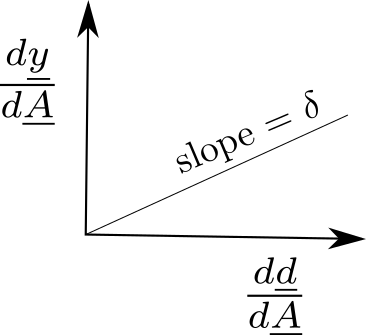
\includegraphics[width=1.5in]
{instrumental/slope-delta.png}
\caption{Effect $\delta$ as slope of line.}
\label{fig-slope-delta}
\end{figure}


\section{More general bnets with IVs}

\begin{figure}[h!]
$$
\begin{array}{ccc}
\xymatrix{
&&\rvu\ar@{-->}[dl]\ar@{-->}[dr]
\\
\rva\ar[r]\ar[drr]
&\rvd\ar[rr]_\delta
&&\rvy\ar[dl]
\\
&&\rvv
}
&&
\xymatrix{
&&\rvu\ar@{-->}[dl]\ar@{-->}[dr]
\\
\rva\ar[r]\ar[drr]
&\rvd&
\rvtd\ar[r]_\delta
&\rvy\ar[dl]
\\
&&\rvv
}
\\
\\
G&&G_{im+}
\end{array}
$$
\caption{The 2 paths in $G_{im+}$
from
IV variable $\rva$
to $\rvy$ are blocked by
not conditioning on colliders $\rvv$
and $\rvd$. Thus,
$
\rvd\perp_{G_{im+}} \rvy =\text{false}, 
\;\; \rva\perp_{G_{im+}} \rvy= \text{true}
$.
}
\label{fig-iv-G-im-blocked}
\end{figure}




\begin{figure}[h!]
$$
\begin{array}{ccc}
\xymatrix{
&&\rvu\ar@{-->}[dl]\ar@{-->}[dr]
\\
\rva\ar[r]
&\rvd\ar[rr]_\delta
&&\rvy
\\
&&\rvv\ar[ur]\ar[ull]
}
&&
\xymatrix{
&&\rvu\ar@{-->}[dl]\ar@{-->}[dr]
\\
\rva\ar[r]
&\rvd
&
\rvtd\ar[r]_\delta
&\rvy
\\
&&\rvv\ar[ur]\ar[ull]
}
\\
\\
G&&G_{im+}
\end{array}
$$
\caption{
There are 2 paths in $G_{im+}$
from
IV variable $\rva$
to $\rvy$. One is
blocked
by not conditioning on the collider $\rvd$
and the other
can be blocked by 
conditioning on $\rvv$. Thus,
$
\rvd\perp_{G_{im+}} \rvy|\rvv =\text{false}, 
\;\; \rva\perp_{G_{im+}} \rvy|\rvv= \text{true}
$.
}
\label{fig-iv-G-im-strata}
\end{figure}

Figs.\ref{fig-iv-G-im-blocked}
and \ref{fig-iv-G-im-strata}
are examples of 
other bnets 
for which the
effect $\delta$
is identifiable
thanks
to the
IV $\rva$.


\section{Instrumental Inequality}
Pearl's instrumental inequality
and related inequalities are discussed in
 Chapter
 \ref{ch-inst-ineq}.


